% ថ្នាក់ទី ១១ (វិទ្យាសាស្ត្រសង្គម) · ជំពូកទី ៣ · មេរៀនទី ២ · សៀវភៅ ទំព័រ ៩០–៩៩
\chapter{រូបមន្តត្រីកោណមាត្រ}

\begin{objBox}[វត្ថុបំណង]
\begin{enumerate}[1]
  \item ស្រាយបញ្ជាក់ រូបមន្តផលបូកមុំឌុបនិងរូបមន្តបម្លែង
  \item ដោះស្រាយចំណោទត្រីកោណមាត្រ ។
\end{enumerate}
\end{objBox}

\section{រូបមន្តផលបូកនិងផលដក}

\subsection{គណនា \texorpdfstring{$\cos(\alpha - \beta)$}{cos(α − β)} និង \texorpdfstring{$\cos(\alpha + \beta)$}{cos(α + β)}}

\begin{example}[ឧទាហរណ៍ ១]
ប្រៀបធៀបកន្សោម $\cos(60^\circ - 30^\circ)$ និង $\cos 60^\circ - \cos 30^\circ$ ។ គេបាន
\[ \cos(60^\circ - 30^\circ) = \cos 30^\circ = \frac{\sqrt{3}}{2} = 0.866 \]
\[ \cos 60^\circ - \cos 30^\circ = \frac{1}{2} - \frac{\sqrt{3}}{2} = \frac{1}{2}(1 - \sqrt{3}) = -0.366 \]
ដូច្នេះ $\cos(60^\circ - 30^\circ) \ne \cos 60^\circ - \cos 30^\circ$ ។
\end{example}

ក្នុងការគណនា $\cos(60^\circ - 45^\circ) = \cos 15^\circ$ គេមិនអាចរក $\cos 15^\circ$ បានដោយងាយនោះទេ ព្រោះ $15^\circ$ មិនមែនជាមុំពិសេស ។ ដូច្នេះគេបង្កើតរូបមន្តដើម្បីងាយស្រួលក្នុងការរកអនុគមន៍ត្រីកោណមាត្រនៃមុំទាំងនោះដូចខាងក្រោម ៖

គេពិនិត្យរង្វង់ត្រីកោណមាត្រដែលមានមុំ $(\overrightarrow{OA}, \overrightarrow{OM}) = \alpha$, មុំ $(\overrightarrow{OA}, \overrightarrow{ON}) = \beta$ និងមុំ $(\overrightarrow{OM}, \overrightarrow{ON}) = \beta - \alpha$ ។
\begin{center}
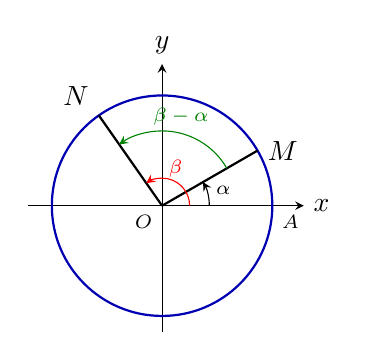
\begin{tikzpicture}[scale=1,>=stealth]
  \draw[->] (-1.7,0) -- (1.8,0) node[right] {$x$};
  \draw[->] (0,-1.6) -- (0,1.8) node[above] {$y$};
  \draw[blue!70!black,thick] (0,0) circle (1.4);
  \draw[thick] (0,0) -- (30:1.4) node[right] {$M$};
  \draw[thick] (0,0) -- (125:1.4) node[above left] {$N$};
  \node[below right] at (1.4,0) {\scriptsize $A$}; \node[below left] at (0,0) {\scriptsize $O$};
  \draw[->,red] (0.35,0) arc (0:125:0.35); \node[red] at (70:0.5) {\scriptsize $\beta$};
  \draw[->] (0.6,0) arc (0:30:0.6); \node at (14:0.8) {\scriptsize $\alpha$};
  \draw[->,green!50!black] (30:0.95) arc (30:125:0.95); \node[green!50!black] at (78:1.15) {\scriptsize $\beta - \alpha$};
\end{tikzpicture}
\end{center}
គេបាន $\overrightarrow{OM}(\cos\alpha, \sin\alpha)$, $\overrightarrow{ON}(\cos\beta, \sin\beta)$ ។ តាមនិយមន័យផលគុណស្កាលែ គេអាចសរសេរ
\[ \overrightarrow{OM} \cdot \overrightarrow{ON} = OM \cdot ON \cdot \cos(\beta - \alpha) = \cos(\beta - \alpha) \]
ព្រោះ $OM = ON = 1$ (កាំរង្វង់ត្រីកោណមាត្រ) និង $\cos(-x) = \cos x$ ។ ម្យ៉ាងទៀតតាមកន្សោមវិភាគផលគុណស្កាលែ គេបាន $\overrightarrow{OM} \cdot \overrightarrow{ON} = \cos\alpha\cos\beta + \sin\alpha\sin\beta$ ។
\begin{formulaBox}[ដូច្នេះ]
\[ \cos(\alpha - \beta) = \cos\alpha\cos\beta + \sin\alpha\sin\beta \quad (1) \]
\end{formulaBox}

\begin{example}[ឧទាហរណ៍ ២]
\[
\begin{aligned}
\cos 15^\circ &= \cos(60^\circ - 45^\circ)\\
&= \cos 60^\circ\cos 45^\circ + \sin 60^\circ\sin 45^\circ\\
&= \frac{1}{2} \times \frac{\sqrt{2}}{2} + \frac{\sqrt{3}}{2} \times \frac{\sqrt{2}}{2} = \frac{\sqrt{2} + \sqrt{6}}{4} \text{ ។}
\end{aligned}
\]
\end{example}

បើគេជំនួស $-\beta$ ដោយ $\beta$ ក្នុងរូបមន្ត $\cos(\alpha - \beta)$ គេបាន $\cos[\alpha - (-\beta)] = \cos\alpha\cos(-\beta) + \sin\alpha\sin(-\beta)$ នាំឱ្យ
\begin{formulaBox}[រូបមន្ត]
\[ \cos(\alpha + \beta) = \cos\alpha\cos\beta - \sin\alpha\sin\beta \quad (2) \]
\end{formulaBox}

\begin{example}[ឧទាហរណ៍ ៣]
\[
\begin{aligned}
\cos\frac{5\pi}{12} &= \cos\left(\frac{\pi}{4} + \frac{\pi}{6}\right) = \cos\frac{\pi}{4}\cos\frac{\pi}{6} - \sin\frac{\pi}{4}\sin\frac{\pi}{6}\\
&= \frac{\sqrt{2}}{2} \times \frac{\sqrt{3}}{2} - \frac{\sqrt{2}}{2} \times \frac{1}{2} = \frac{\sqrt{6} - \sqrt{2}}{4} \text{ ។}
\end{aligned}
\]
\end{example}

\subsection{គណនា \texorpdfstring{$\sin(\alpha - \beta)$}{sin(α − β)} និង \texorpdfstring{$\sin(\alpha + \beta)$}{sin(α + β)}}

តាមលក្ខណៈមុំបំពេញ គេបាន $\sin(\alpha + \beta) = \cos\left[\dfrac{\pi}{2} - (\alpha + \beta)\right] = \cos\left[\left(\dfrac{\pi}{2} - \alpha\right) - \beta\right]$ ។

តាមរូបមន្ត $(1)$ \ $\sin(\alpha + \beta) = \cos\left(\dfrac{\pi}{2} - \alpha\right)\cos\beta + \sin\left(\dfrac{\pi}{2} - \alpha\right)\sin\beta$ ។

តែ $\cos\left(\dfrac{\pi}{2} - \alpha\right) = \sin\alpha$ និង $\sin\left(\dfrac{\pi}{2} - \alpha\right) = \cos\alpha$ ។
\begin{formulaBox}[ដូច្នេះ]
\[ \sin(\alpha + \beta) = \sin\alpha\cos\beta + \sin\beta\cos\alpha \quad (3) \]
\end{formulaBox}

\begin{example}[ឧទាហរណ៍ ៤]
\[
\begin{aligned}
\sin 75^\circ &= \sin(45^\circ + 30^\circ)\\
&= \sin 45^\circ\cos 30^\circ + \cos 45^\circ\sin 30^\circ\\
&= \frac{\sqrt{2}}{2} \times \frac{\sqrt{3}}{2} + \frac{\sqrt{2}}{2} \times \frac{1}{2} = \frac{\sqrt{6} + \sqrt{2}}{4} \text{ ។}
\end{aligned}
\]
\end{example}

បើយើងជំនួស $\beta$ ដោយ $(-\beta)$ ក្នុងរូបមន្ត $(3)$ គេបាន $\sin(\alpha - \beta) = \sin[\alpha + (-\beta)]$
\[ \sin(\alpha - \beta) = \sin\alpha\cos(-\beta) + \sin(-\beta)\cos\alpha \]
ដោយ $\cos(-\beta) = \cos\beta$ និង $\sin(-\beta) = -\sin\beta$ ។
\begin{formulaBox}[ដូច្នេះ]
\[ \sin(\alpha - \beta) = \sin\alpha\cos\beta - \sin\beta\cos\alpha \quad (4) \]
\end{formulaBox}

\begin{example}[ឧទាហរណ៍ ៥]
\[
\begin{aligned}
\sin\frac{\pi}{12} &= \sin\left(\frac{\pi}{4} - \frac{\pi}{6}\right) = \sin\frac{\pi}{4}\cos\frac{\pi}{6} - \sin\frac{\pi}{6}\cos\frac{\pi}{4}\\
&= \frac{\sqrt{2}}{2} \times \frac{\sqrt{3}}{2} - \frac{1}{2} \times \frac{\sqrt{2}}{2} = \frac{\sqrt{6} - \sqrt{2}}{4} \text{ ។}
\end{aligned}
\]
\end{example}

\begin{example}[លំហាត់គំរូ ១]
គណនា $\dfrac{\sin 9^\circ\cos 39^\circ - \cos 9^\circ\sin 39^\circ}{\cos\frac{3\pi}{7}\cos\frac{5\pi}{28} + \sin\frac{3\pi}{7}\sin\frac{5\pi}{28}}$ ។
\end{example}
\ans
\[
\begin{aligned}
\frac{\sin 9^\circ\cos 39^\circ - \cos 9^\circ\sin 39^\circ}{\cos\frac{3\pi}{7}\cos\frac{5\pi}{28} + \sin\frac{3\pi}{7}\sin\frac{5\pi}{28}} &= \frac{\sin(9^\circ - 39^\circ)}{\cos\left(\frac{12\pi}{28} - \frac{5\pi}{28}\right)}\\
&= \frac{\sin(-30^\circ)}{\cos\frac{\pi}{4}} = -\frac{1}{\sqrt{2}} = -\frac{\sqrt{2}}{2} \text{ ។}
\end{aligned}
\]

\begin{example}[លំហាត់គំរូ ២]
បង្ហាញថា $\sin\alpha + \cos\alpha = \sqrt{2}\sin\left(\alpha + \dfrac{\pi}{4}\right)$ ។
\end{example}
\ans
\[
\begin{aligned}
\sin\alpha + \cos\alpha &= \sqrt{2}\left(\frac{\sqrt{2}}{2}\sin\alpha + \frac{\sqrt{2}}{2}\cos\alpha\right)\\
&= \sqrt{2}\left(\sin\alpha\cos\frac{\pi}{4} + \sin\frac{\pi}{4}\cos\alpha\right) = \sqrt{2}\sin\left(\alpha + \frac{\pi}{4}\right) \text{ ។}
\end{aligned}
\]

\begin{pro}
\begin{enumerate}[1]
  \item គណនា $\sin 105^\circ$, $\cos 105^\circ$, $\cos\dfrac{\pi}{12}$ ។
  \item បង្ហាញថា $\dfrac{\sin(\alpha - \beta)}{\cos\alpha\cos\beta} + \dfrac{\sin(\beta - \theta)}{\cos\beta\cos\theta} + \dfrac{\sin(\theta - \alpha)}{\cos\theta\cos\alpha} = 0$ ។
\end{enumerate}
\ans
\begin{enumerate}[1]
  \item $\sin 105^\circ = \dfrac{\sqrt{6} + \sqrt{2}}{4}$, \ $\cos 105^\circ = \dfrac{\sqrt{2} - \sqrt{6}}{4}$, \ $\cos\dfrac{\pi}{12} = \dfrac{\sqrt{6} + \sqrt{2}}{4}$ ។
  \item ប្រើ $\dfrac{\sin(\alpha - \beta)}{\cos\alpha\cos\beta} = \tan\alpha - \tan\beta$ ។
\end{enumerate}
\end{pro}

\subsection{គណនា \texorpdfstring{$\tan(\alpha + \beta)$}{tan(α + β)} និង \texorpdfstring{$\tan(\alpha - \beta)$}{tan(α − β)}}

គេមាន $\tan(\alpha + \beta) = \dfrac{\sin(\alpha + \beta)}{\cos(\alpha + \beta)}$ ដោយប្រើរូបមន្ត $(2)$ និង $(3)$ គេបាន $\tan(\alpha + \beta) = \dfrac{\sin\alpha\cos\beta + \sin\beta\cos\alpha}{\cos\alpha\cos\beta - \sin\alpha\sin\beta}$ ។

ឧបមាថា $\cos\alpha \ne 0$, $\cos\beta \ne 0$, $\cos(\alpha + \beta) \ne 0$ ។ គេចែកតួទាំងពីរនៃផលធៀបនឹង $\cos\alpha\cos\beta$ គេបាន
\[ \tan(\alpha + \beta) = \frac{\frac{\sin\alpha\cos\beta}{\cos\alpha\cos\beta} + \frac{\sin\beta\cos\alpha}{\cos\alpha\cos\beta}}{\frac{\cos\alpha\cos\beta}{\cos\alpha\cos\beta} - \frac{\sin\alpha\sin\beta}{\cos\alpha\cos\beta}} \]
\begin{formulaBox}[ឬ]
\[ \tan(\alpha + \beta) = \frac{\tan\alpha + \tan\beta}{1 - \tan\alpha\tan\beta} \quad (5) \]
\end{formulaBox}

\begin{example}[ឧទាហរណ៍ ៦]
\[
\begin{aligned}
\tan 105^\circ &= \tan(60^\circ + 45^\circ) = \frac{\tan 60^\circ + \tan 45^\circ}{1 - \tan 60^\circ\tan 45^\circ}\\
&= \frac{\sqrt{3} + 1}{1 - \sqrt{3} \times 1} = \frac{\sqrt{3} + 1}{1 - \sqrt{3}} \text{ ។}
\end{aligned}
\]
\end{example}

បើគេជំនួស $\beta$ ដោយ $(-\beta)$ ក្នុងរូបមន្ត $\tan(\alpha + \beta)$ ។ គេបាន $\tan[\alpha + (-\beta)] = \dfrac{\tan\alpha + \tan(-\beta)}{1 - \tan\alpha\tan(-\beta)}$
\begin{formulaBox}[រូបមន្ត]
\[ \tan(\alpha - \beta) = \frac{\tan\alpha - \tan\beta}{1 + \tan\alpha\tan\beta} \quad (6) \]
\end{formulaBox}
រូបមន្តនេះកំណត់បានលុះត្រាតែ $\alpha \ne \dfrac{\pi}{2} + k\pi$, $\beta \ne \dfrac{\pi}{2} + k\pi$, $(\alpha - \beta) \ne \dfrac{\pi}{2} + k\pi$, $k \in \mathbb{Z}$ ។

\begin{example}[ឧទាហរណ៍ ៧]
\[
\begin{aligned}
\tan\frac{\pi}{12} &= \tan\left(\frac{\pi}{4} - \frac{\pi}{6}\right) = \frac{\tan\frac{\pi}{4} - \tan\frac{\pi}{6}}{1 + \tan\frac{\pi}{4}\tan\frac{\pi}{6}}\\
&= \frac{1 - \frac{\sqrt{3}}{3}}{1 + 1 \times \frac{\sqrt{3}}{3}} = \frac{3 - \sqrt{3}}{3 + \sqrt{3}}\\
&= 2 - \sqrt{3} \text{ ។}
\end{aligned}
\]
\end{example}

\begin{example}[លំហាត់គំរូ ៣]
គេឱ្យ $0 < \alpha < \dfrac{\pi}{2}$, $-\dfrac{\pi}{2} < \beta < 0$ និង $\tan\alpha = 2$, $\tan\beta = -3$ ។ គណនា $\tan(\alpha - \beta)$ ។
\end{example}
\ans
\[ \tan(\alpha - \beta) = \frac{\tan\alpha - \tan\beta}{1 + \tan\alpha\tan\beta} = \frac{2 - (-3)}{1 + 2(-3)} = \frac{5}{-5} = -1 \text{ ។} \]

\begin{example}[លំហាត់គំរូ ៤]
សម្រួលកន្សោម $\dfrac{\tan 3\theta - \tan\theta}{1 + \tan\theta\tan 3\theta} + \cot\left(\dfrac{\pi}{2} + 2\theta\right)$ ។
\end{example}
\ans
គេមាន $\dfrac{\tan 3\theta - \tan\theta}{1 + \tan\theta\tan 3\theta} = \tan(3\theta - \theta) = \tan 2\theta$ និង $\cot\left(\dfrac{\pi}{2} + 2\theta\right) = -\tan 2\theta$ ។

ដូច្នេះ $\dfrac{\tan 3\theta - \tan\theta}{1 + \tan\theta\tan 3\theta} + \cot\left(\dfrac{\pi}{2} + 2\theta\right) = \tan 2\theta - \tan 2\theta = 0$ ។

\begin{pro}
\begin{enumerate}[1]
  \item គណនា $\tan(a + b + c)$ ដោយប្រើរូបមន្ត $\tan(\alpha + \beta)$ ។
  \item ផ្ទៀងផ្ទាត់សមភាព $\dfrac{1 - \tan\theta}{1 + \tan\theta} = \tan\left(\dfrac{\pi}{4} - \theta\right)$ ។
\end{enumerate}
\ans
\begin{enumerate}[1]
  \item $\tan(a + b + c) = \dfrac{\tan a + \tan b + \tan c - \tan a\tan b\tan c}{1 - \tan a\tan b - \tan b\tan c - \tan c\tan a}$ ។
\end{enumerate}
\end{pro}

\section{អនុគមន៍រូបមន្តផលបូក}

\subsection{រូបមន្តមុំឌុប}

\begin{itemize}
  \item គេឱ្យ $\alpha = \beta$ ជំនួស $\beta$ ដោយ $\alpha$ ក្នុងរូបមន្ត $\sin(\alpha + \beta)$ គេបាន $\sin 2\alpha = \sin(\alpha + \alpha) = \sin\alpha\cos\alpha + \cos\alpha\sin\alpha = 2\sin\alpha\cos\alpha$ ។
  \begin{formulaBox}[ដូច្នេះ]
  \[ \sin 2\alpha = 2\sin\alpha\cos\alpha \quad (7) \]
  \end{formulaBox}
  \item បើគេជំនួស $\beta$ ដោយ $\alpha$ ទៅក្នុងរូបមន្ត $\cos(\alpha + \beta)$ គេបាន $\cos 2\alpha = \cos(\alpha + \alpha) = \cos\alpha\cos\alpha - \sin\alpha\sin\alpha = \cos^2\alpha - \sin^2\alpha$ ។

  គេសង្កេតឃើញថា $\cos^2\alpha = 1 - \sin^2\alpha$ និង $\sin^2\alpha = 1 - \cos^2\alpha$ ។ គេបាន $\cos 2\alpha = (1 - \sin^2\alpha) - \sin^2\alpha = 1 - 2\sin^2\alpha$ និង $\cos 2\alpha = \cos^2\alpha - (1 - \cos^2\alpha) = 2\cos^2\alpha - 1$ ។
  \begin{formulaBox}[ដូច្នេះ]
  \[
\begin{gathered}
\cos 2\alpha = \cos^2\alpha - \sin^2\alpha = 1 - 2\sin^2\alpha = 2\cos^2\alpha - 1\\
(8)
\end{gathered}
\]
  \end{formulaBox}
  \item បើគេជំនួស $\beta$ ដោយ $\alpha$ ទៅក្នុងរូបមន្ត $\tan(\alpha + \beta)$ គេបាន $\tan 2\alpha = \tan(\alpha + \alpha) = \dfrac{\tan\alpha + \tan\alpha}{1 - \tan\alpha\tan\alpha} = \dfrac{2\tan\alpha}{1 - \tan^2\alpha}$ ។
  \begin{formulaBox}[ដូច្នេះ]
  \[ \tan 2\alpha = \frac{2\tan\alpha}{1 - \tan^2\alpha} \quad (9) \]
  \end{formulaBox}
\end{itemize}

\begin{example}[ឧទាហរណ៍ ៨]
រក $\sin 2\alpha$, $\cos 2\alpha$ និង $\tan 2\alpha$ បើ $\cos\alpha = -\dfrac{4}{5}$ និង $\dfrac{\pi}{2} < \alpha < \pi$ ។

ដោយ $\dfrac{\pi}{2} < \alpha < \pi$ នាំឱ្យ $\sin\alpha > 0$ គេបាន $\sin^2\alpha = 1 - \cos^2\alpha$, $\sin\alpha = \sqrt{1 - \cos^2\alpha}$
\[ \sin\alpha = \sqrt{1 - \left(-\frac{4}{5}\right)^2} = \frac{3}{5} \]
ដូច្នេះ
\[
\begin{gathered}
\sin 2\alpha = 2\sin\alpha\cos\alpha = 2 \times \frac{3}{5} \times \left(-\frac{4}{5}\right) = -\frac{24}{25},\\
\cos 2\alpha = 2\cos^2\alpha - 1 = 2 \times \left(-\frac{4}{5}\right)^2 - 1 = \frac{7}{25}
\end{gathered}
\]
គេបាន $\tan\alpha = \dfrac{\sin\alpha}{\cos\alpha} = -\dfrac{3}{4}$ នាំឱ្យ
\[ \tan 2\alpha = \frac{2\tan\alpha}{1 - \tan^2\alpha} = \frac{2 \times \left(-\frac{3}{4}\right)}{1 - \left(-\frac{3}{4}\right)^2} = -\frac{24}{7} \]
គេអាចរក $\tan 2\alpha = \dfrac{\sin 2\alpha}{\cos 2\alpha} = -\dfrac{24}{7}$ ។
\end{example}

\begin{example}[ឧទាហរណ៍ ៩]
គណនា $\sin 3\alpha$ និង $\cos 3\alpha$ ។
\[
\begin{aligned}
\sin 3\alpha &= \sin(2\alpha + \alpha) = \sin 2\alpha\cos\alpha + \sin\alpha\cos 2\alpha\\
&= 2\sin\alpha\cos\alpha\cos\alpha + \sin\alpha(1 - 2\sin^2\alpha)\\
&= 2\sin\alpha\cos^2\alpha + \sin\alpha - 2\sin^3\alpha\\
&= 2\sin\alpha(1 - \sin^2\alpha) + \sin\alpha - 2\sin^3\alpha\\
&= 2\sin\alpha - 2\sin^3\alpha + \sin\alpha - 2\sin^3\alpha\\
&= 3\sin\alpha - 4\sin^3\alpha
\end{aligned}
\]
\end{example}
\begin{formulaBox}[ដូច្នេះ]
\[ \sin 3\alpha = 3\sin\alpha - 4\sin^3\alpha \quad (10) \]
\end{formulaBox}
$\cos 3\alpha = \cos(2\alpha + \alpha) = \cos 2\alpha\cos\alpha - \sin 2\alpha\sin\alpha$ ប្រើ $\cos 2\alpha$ និង $\sin 2\alpha$
\begin{formulaBox}[ដូច្នេះ]
\[ \cos 3\alpha = 4\cos^3\alpha - 3\cos\alpha \quad (11) \]
\end{formulaBox}

\begin{example}[លំហាត់គំរូ ៥]
ដោយប្រើ $\sin 3x$ និង $\cos 3x$ គណនា $\sin 4x$ ។
\end{example}
\ans
\[
\begin{aligned}
\sin 4x &= \sin(3x + x) = \sin 3x\cos x + \sin x\cos 3x\\
&= (3\sin x - 4\sin^3 x)\cos x\\
&\quad + \sin x(4\cos^3 x - 3\cos x)\\
&= 4(\cos^3 x\sin x - \sin^3 x\cos x) \text{ ។}
\end{aligned}
\]

\begin{pro}
បង្ហាញថា $\dfrac{1 - 2\sin^2\alpha}{2\cot\left(\frac{\pi}{4} + \alpha\right)\cos^2\left(\frac{\pi}{4} - \alpha\right)} = 1$ ។
\end{pro}

\subsection{រូបមន្តកន្លះមុំ}

\begin{itemize}
  \item បើគេជំនួស $2\alpha$ ដោយ $\alpha$ និង $\alpha$ ដោយ $\dfrac{\alpha}{2}$ ទៅក្នុងរូបមន្ត $\sin 2\alpha = 2\sin\alpha\cos\alpha$, $\cos^2\alpha = \dfrac{1 + \cos 2\alpha}{2}$, $\sin^2\alpha = \dfrac{1 - \cos 2\alpha}{2}$ និង $\tan^2\alpha = \dfrac{1 - \cos 2\alpha}{1 + \cos 2\alpha}$ គេបាន
  \begin{formulaBox}[រូបមន្ត]
  \[
  \begin{aligned}
  \sin\alpha &= 2\sin\frac{\alpha}{2}\cos\frac{\alpha}{2}, & \cos^2\frac{\alpha}{2} &= \frac{1 + \cos\alpha}{2}\\
  \sin^2\frac{\alpha}{2} &= \frac{1 - \cos\alpha}{2}, & \tan^2\frac{\alpha}{2} &= \frac{1 - \cos\alpha}{1 + \cos\alpha} \qquad (12)
  \end{aligned}
  \]
  \end{formulaBox}
  រូបមន្តម្យ៉ាងទៀតរបស់ $\tan\dfrac{\alpha}{2}$ គឺ
  \[ \tan x = \frac{\sin x}{\cos x} = \frac{2\sin x\cos x}{2\cos x\cos x} = \frac{\sin 2x}{2\cos^2 x} = \frac{\sin 2x}{1 + \cos 2x} \]
  \item បើគេជំនួស $x$ ដោយ $\dfrac{\alpha}{2}$ និង $\alpha = 2x$ គេបាន
  \begin{formulaBox}[រូបមន្ត]
  \[ \tan\frac{\alpha}{2} = \frac{\sin\alpha}{1 + \cos\alpha} \quad (13) \]
  \end{formulaBox}
\end{itemize}

បើគេជំនួស $2\alpha$ ដោយ $\alpha$ និង $\alpha$ ដោយ $\dfrac{\alpha}{2}$ ទៅក្នុងរូបមន្ត $(7)$, $(8)$ និង $(9)$ គេបាន ៖
\[
\begin{gathered}
\cos\alpha = \cos^2\frac{\alpha}{2} - \sin^2\frac{\alpha}{2}, \quad \sin\alpha = 2\sin\frac{\alpha}{2}\cos\frac{\alpha}{2},\\
\tan\alpha = \frac{2\tan\frac{\alpha}{2}}{1 - \tan^2\frac{\alpha}{2}} \text{ ។}
\end{gathered}
\]
ដោយ $\cos^2\dfrac{\alpha}{2} + \sin^2\dfrac{\alpha}{2} = 1$ គេអាចសរសេរ
\[
\begin{gathered}
\cos\alpha = \frac{\cos^2\frac{\alpha}{2} - \sin^2\frac{\alpha}{2}}{\cos^2\frac{\alpha}{2} + \sin^2\frac{\alpha}{2}},\\
\sin\alpha = \frac{2\sin\frac{\alpha}{2}\cos\frac{\alpha}{2}}{\cos^2\frac{\alpha}{2} + \sin^2\frac{\alpha}{2}}
\end{gathered}
\]
គេចែកភាគយកនិងភាគបែងកន្សោមទាំងពីរនឹង $\cos^2\dfrac{\alpha}{2}$ ដែល $\cos\dfrac{\alpha}{2} \ne 0$ គេបាន
\[
\begin{gathered}
\cos\alpha = \frac{1 - \tan^2\frac{\alpha}{2}}{1 + \tan^2\frac{\alpha}{2}},\\
\sin\alpha = \frac{2\tan\frac{\alpha}{2}}{1 + \tan^2\frac{\alpha}{2}} \text{ ។}
\end{gathered}
\]
បើគេឱ្យ $\tan\dfrac{\alpha}{2} = t$
\begin{formulaBox}[គេបានរូបមន្ត]
\[
\begin{gathered}
\cos\alpha = \frac{1 - t^2}{1 + t^2}, \quad \sin\alpha = \frac{2t}{1 + t^2}, \quad \tan\alpha = \frac{2t}{1 - t^2}\\
(14)
\end{gathered}
\]
\end{formulaBox}

\begin{example}[ឧទាហរណ៍ ១០]
គណនា $\sin 22^\circ 30'$, $\sin\dfrac{\pi}{12}$ និង $\tan\dfrac{3\pi}{8}$ ។

គេដឹងថាមុំ $22^\circ 30'$ នៅក្នុងកាដ្រង់ទី I ដូច្នេះ $\sin$ និង $\cos$ មានតម្លៃវិជ្ជមាន ។ គេបាន
\[
\begin{aligned}
\sin 22^\circ 30' &= \sin\frac{45^\circ}{2} = \sqrt{\frac{1 - \cos 45^\circ}{2}} = \sqrt{\frac{1 - \frac{\sqrt{2}}{2}}{2}}\\
&= \frac{\sqrt{2 - \sqrt{2}}}{2} \text{ ។}
\end{aligned}
\]
\[ \sin^2\frac{\pi}{12} = \sin^2\left(\frac{1}{2} \times \frac{\pi}{6}\right) = \frac{1 - \cos\frac{\pi}{6}}{2} = \frac{1 - \frac{\sqrt{3}}{2}}{2} = \frac{2 - \sqrt{3}}{4} \]
ដោយ $\sin\dfrac{\pi}{12} > 0$ នាំឱ្យ $\sin\dfrac{\pi}{12} = \dfrac{\sqrt{2 - \sqrt{3}}}{2}$ ។
\[
\begin{aligned}
\tan\frac{3\pi}{8} &= \tan\left(\frac{1}{2} \times \frac{3\pi}{4}\right) = \frac{\sin\frac{3\pi}{4}}{1 + \cos\frac{3\pi}{4}} = \frac{\frac{\sqrt{2}}{2}}{1 - \frac{\sqrt{2}}{2}}\\
&= \frac{\sqrt{2}}{2 - \sqrt{2}} = \sqrt{2} + 1 \text{ ។}
\end{aligned}
\]
\end{example}

\begin{example}[ឧទាហរណ៍ ១១]
ផ្ទៀងផ្ទាត់សមភាព $\dfrac{1 - \cos x}{\sin x} = \tan\dfrac{x}{2}$ ។

តាង $\tan\dfrac{x}{2} = t$ គេបាន
\[ \frac{1 - \cos x}{\sin x} = \frac{1 - \frac{1 - t^2}{1 + t^2}}{\frac{2t}{1 + t^2}} = \frac{\frac{1 + t^2 - 1 + t^2}{1 + t^2}}{\frac{2t}{1 + t^2}} = \frac{2t^2}{2t} = t = \tan\frac{x}{2} \text{ ។} \]
\end{example}

\begin{example}[លំហាត់គំរូ ៦]
គេមាន $\cos\alpha = -\dfrac{3}{5}$ ហើយ $\dfrac{\pi}{2} < \alpha < \pi$ ។ គណនា $\sin\dfrac{\alpha}{2}$ និង $\cos\dfrac{\alpha}{2}$ ។
\end{example}
\ans
ដោយ $\dfrac{\pi}{2} < \alpha < \pi$ នោះនាំឱ្យ $\sin\alpha > 0$, $\cos\alpha < 0$ ហើយ $\dfrac{\pi}{4} < \dfrac{\alpha}{2} < \dfrac{\pi}{2}$ ។ គេបាន $\sin^2\alpha = 1 - \cos^2\alpha = 1 - \left(-\dfrac{3}{5}\right)^2 = \dfrac{16}{25}$ ។ ដូច្នេះ $\sin\alpha = \dfrac{4}{5}$ ។
\[
\begin{gathered}
\sin\frac{\alpha}{2} = \sqrt{\frac{1 - \cos\alpha}{2}} = \sqrt{\frac{1 + \frac{3}{5}}{2}} = \sqrt{\frac{4}{5}} = \frac{2\sqrt{5}}{5},\\
\cos\frac{\alpha}{2} = \sqrt{\frac{1 + \cos\alpha}{2}} = \sqrt{\frac{1 - \frac{3}{5}}{2}} = \sqrt{\frac{1}{5}} = \frac{\sqrt{5}}{5} \text{ ។}
\end{gathered}
\]

\begin{pro}
គណនា $\tan\dfrac{\alpha}{2}$ ដោយស្គាល់ $\tan\alpha = \dfrac{24}{7}$ និង $180^\circ < \alpha < 270^\circ$ ។
\ans
$\cos\alpha = -\dfrac{7}{25}$, $\sin\alpha = -\dfrac{24}{25}$ ។ \ $\tan\dfrac{\alpha}{2} = \dfrac{\sin\alpha}{1 + \cos\alpha} = -\dfrac{4}{3}$ ។
\end{pro}

\section{រូបមន្តបម្លែង}

\subsection{បម្លែងពីផលគុណទៅជាផលបូក}

តាមរូបមន្តផលបូកនិងផលដកខាងក្រោម ៖
\[
\begin{gathered}
\cos(\alpha - \beta) = \cos\alpha\cos\beta + \sin\alpha\sin\beta \quad (1),\\
\cos(\alpha + \beta) = \cos\alpha\cos\beta - \sin\alpha\sin\beta \quad (2)
\end{gathered}
\]
\begin{itemize}
  \item បូករូបមន្ត $(1)$ និង $(2)$ គេបាន $\cos(\alpha + \beta) + \cos(\alpha - \beta) = 2\cos\alpha\cos\beta$
  \item ដករូបមន្ត $(1)$ និង $(2)$ គេបាន $\cos(\alpha + \beta) - \cos(\alpha - \beta) = -2\sin\alpha\sin\beta$ ។
\end{itemize}
\[
\begin{gathered}
\sin(\alpha + \beta) = \sin\alpha\cos\beta + \sin\beta\cos\alpha \quad (3),\\
\sin(\alpha - \beta) = \sin\alpha\cos\beta - \sin\beta\cos\alpha \quad (4)
\end{gathered}
\]
\begin{itemize}
  \item បូករូបមន្ត $(3)$ និង $(4)$ គេបាន $\sin(\alpha + \beta) + \sin(\alpha - \beta) = 2\sin\alpha\cos\beta$
  \item ដករូបមន្ត $(3)$ និង $(4)$ គេបាន $\sin(\alpha + \beta) - \sin(\alpha - \beta) = 2\sin\beta\cos\alpha$ ។
\end{itemize}
\begin{formulaBox}[ដូច្នេះ គេបានរូបមន្ត]
\[
\begin{aligned}
\cos\alpha\cos\beta &= \frac{1}{2}[\cos(\alpha + \beta) + \cos(\alpha - \beta)]\\
\sin\alpha\sin\beta &= \frac{1}{2}[\cos(\alpha - \beta) - \cos(\alpha + \beta)]\\
\sin\alpha\cos\beta &= \frac{1}{2}[\sin(\alpha + \beta) + \sin(\alpha - \beta)]\\
\sin\beta\cos\alpha &= \frac{1}{2}[\sin(\alpha + \beta) - \sin(\alpha - \beta)]
\end{aligned}
\]
\end{formulaBox}

\begin{example}[ឧទាហរណ៍ ១២]
គណនា $\cos 75^\circ\cos 45^\circ$ ។
\[
\begin{aligned}
\cos 75^\circ\cos 45^\circ &= \frac{1}{2}[\cos(75^\circ + 45^\circ) + \cos(75^\circ - 45^\circ)]\\
&= \frac{1}{2}(\cos 120^\circ + \cos 30^\circ)\\
&= \frac{1}{2}\left(-\frac{1}{2} + \frac{\sqrt{3}}{2}\right)\\
&= \frac{\sqrt{3} - 1}{4} \text{ ។}
\end{aligned}
\]
\end{example}

\begin{example}[ឧទាហរណ៍ ១៣]
\[
\begin{aligned}
\sin\frac{5\pi}{12}\sin\frac{\pi}{4} &= \frac{1}{2}\left[\cos\left(\frac{5\pi}{12} - \frac{\pi}{4}\right) - \cos\left(\frac{5\pi}{12} + \frac{\pi}{4}\right)\right]\\
&= \frac{1}{2}\left[\cos\frac{\pi}{6} - \cos\frac{2\pi}{3}\right]\\
&= \frac{1}{2}\left[\frac{\sqrt{3}}{2} - \left(-\frac{1}{2}\right)\right] = \frac{\sqrt{3} + 1}{4} \text{ ។}
\end{aligned}
\]
\end{example}

\subsection{បម្លែងពីផលបូកទៅជាផលគុណ}

តាង $\alpha + \beta = p$, $\alpha - \beta = q$ គេទាញបាន $\alpha = \dfrac{p + q}{2}$ និង $\beta = \dfrac{p - q}{2}$ ។ ជំនួស $\alpha$ និង $\beta$ ទៅក្នុងរូបមន្តខាងលើ គេបាន
\begin{formulaBox}[រូបមន្ត]
\[
\begin{aligned}
\cos p + \cos q &= 2\cos\frac{p + q}{2}\cos\frac{p - q}{2}\\
\cos p - \cos q &= -2\sin\frac{p + q}{2}\sin\frac{p - q}{2}\\
\sin p + \sin q &= 2\sin\frac{p + q}{2}\cos\frac{p - q}{2}\\
\sin p - \sin q &= 2\sin\frac{p - q}{2}\cos\frac{p + q}{2}
\end{aligned}
\]
\end{formulaBox}
ដូចគ្នាដែរគេបាន
\[ \tan p + \tan q = \frac{\sin p}{\cos p} + \frac{\sin q}{\cos q} = \frac{\sin p\cos q + \sin q\cos p}{\cos p\cos q} = \frac{\sin(p + q)}{\cos p\cos q} \text{ ។} \]
ជំនួស $q$ ដោយ $-q$ គេបាន $\tan p - \tan q = \dfrac{\sin(p - q)}{\cos p\cos q}$ ។ ធ្វើតាមវិធីដូចខាងលើ គេបាន $\cot p + \cot q = \dfrac{\sin(p + q)}{\sin p\sin q}$ និង $\cot p - \cot q = \dfrac{\sin(q - p)}{\sin p\sin q}$ ។
\begin{formulaBox}[ដូច្នេះ]
\[
\begin{aligned}
\tan p + \tan q &= \frac{\sin(p + q)}{\cos p\cos q}, & \cot p + \cot q &= \frac{\sin(p + q)}{\sin p\sin q}\\
\tan p - \tan q &= \frac{\sin(p - q)}{\cos p\cos q}, & \cot p - \cot q &= \frac{\sin(q - p)}{\sin p\sin q}
\end{aligned}
\]
\end{formulaBox}

\begin{example}[ឧទាហរណ៍ ១៤]
\[
\begin{aligned}
\sin 105^\circ + \sin 15^\circ &= 2\sin\frac{105^\circ + 15^\circ}{2}\cos\frac{105^\circ - 15^\circ}{2}\\
&= 2\sin 60^\circ\cos 45^\circ = 2 \times \frac{\sqrt{3}}{2} \times \frac{\sqrt{2}}{2} = \frac{\sqrt{6}}{2} \text{ ។}
\end{aligned}
\]
\end{example}

\begin{example}[ឧទាហរណ៍ ១៥]
សរសេរជាផលគុណនៃ $1 + \cos\alpha + \cos 2\alpha$ ។ គេបាន
\[
\begin{aligned}
1 + \cos\alpha + \cos 2\alpha &= 1 + \cos 2\alpha + \cos\alpha = 2\cos^2\alpha + \cos\alpha\\
&= 2\cos\alpha\left(\cos\alpha + \frac{1}{2}\right)\\
&= 2\cos\alpha\left(\cos\alpha + \cos\frac{\pi}{3}\right)\\
&= 4\cos\alpha\cos\left(\frac{\alpha}{2} + \frac{\pi}{6}\right)\cos\left(\frac{\alpha}{2} - \frac{\pi}{6}\right) \text{ ។}
\end{aligned}
\]
\end{example}

\begin{example}[លំហាត់គំរូ ៧]
ផ្ទៀងផ្ទាត់សមភាព $2\left(\dfrac{1}{\sin 2\alpha} + \cot 2\alpha\right) = \cot\dfrac{\alpha}{2} - \tan\dfrac{\alpha}{2}$ ។
\end{example}
\ans
\[
\begin{aligned}
2\left(\frac{1}{\sin 2\alpha} + \cot 2\alpha\right) &= 2\left(\frac{1}{\sin 2\alpha} + \frac{\cos 2\alpha}{\sin 2\alpha}\right)\\
&= 2\left(\frac{2\cos^2\alpha}{2\sin\alpha\cos\alpha}\right)\\
&= \frac{2\cos\alpha}{\sin\alpha}\\
&= \frac{2\left(\cos^2\frac{\alpha}{2} - \sin^2\frac{\alpha}{2}\right)}{2\sin\frac{\alpha}{2}\cos\frac{\alpha}{2}}\\
&= \frac{\cos^2\frac{\alpha}{2}}{\sin\frac{\alpha}{2}\cos\frac{\alpha}{2}} - \frac{\sin^2\frac{\alpha}{2}}{\sin\frac{\alpha}{2}\cos\frac{\alpha}{2}}\\
&= \cot\frac{\alpha}{2} - \tan\frac{\alpha}{2} \text{ ។}
\end{aligned}
\]

\begin{example}[លំហាត់គំរូ ៨]
គេមាន $A$, $B$, $C$ ជាមុំក្នុងត្រីកោណមួយ ។ បង្ហាញថា $\sin A + \sin B + \sin C = 4\cos\dfrac{A}{2}\cos\dfrac{B}{2}\cos\dfrac{C}{2}$ ។
\end{example}
\ans
គេមាន $\sin A + \sin B + \sin C = 2\sin\dfrac{A + B}{2}\cos\dfrac{A - B}{2} + 2\sin\dfrac{C}{2}\cos\dfrac{C}{2}$ ។

ដោយ $A + B + C = \pi \Rightarrow \dfrac{A + B}{2} = \dfrac{\pi}{2} - \dfrac{C}{2}$ ។ ដូច្នេះ $\sin\dfrac{A + B}{2} = \cos\dfrac{C}{2}$, \ $\cos\dfrac{A + B}{2} = \sin\dfrac{C}{2}$ ។ គេបាន
\[
\begin{aligned}
\sin A + \sin B + \sin C &= 2\cos\frac{C}{2}\cos\frac{A - B}{2}\\
&\quad + 2\cos\frac{A + B}{2}\cos\frac{C}{2}\\
&= 2\cos\frac{C}{2}\left(\cos\frac{A - B}{2} + \cos\frac{A + B}{2}\right)\\
&= 4\cos\frac{A}{2}\cos\frac{B}{2}\cos\frac{C}{2} \text{ ។}
\end{aligned}
\]

\begin{pro}
$A$, $B$, $C$ ជាមុំក្នុងត្រីកោណមួយ ។ បង្ហាញថា $\cos A + \cos B + \cos C = 1 + 4\sin\dfrac{A}{2}\sin\dfrac{B}{2}\sin\dfrac{C}{2}$ ។
\end{pro}

\section*{លំហាត់អនុវត្តន៍}
\begin{enumerate}[1]
  \item គេមាន $\sin\alpha = \dfrac{1}{2}$ $\left(0 < \alpha < \dfrac{\pi}{2}\right)$, $\sin\beta = \dfrac{1}{3}$ $\left(\dfrac{\pi}{2} < \beta < \pi\right)$ ។ គណនា $\sin(\alpha + \beta)$, $\cos(\alpha - \beta)$, $\tan(\alpha - \beta)$ និង $\cot(\alpha - \beta)$ ។
  \item គេមាន $\cos\theta = -\dfrac{2}{3}$, $\left(\dfrac{\pi}{2} < \theta < \pi\right)$ ។ គណនា $\cos 2\theta$, $\sin\dfrac{\theta}{2}$, $\sin 3\theta$ ។
  \item គេមាន $t = \tan\dfrac{\theta}{2}$ $(t \ne \pm 1)$, $\sin\theta = \dfrac{2t}{1 + t^2}$, $\cos\theta = \dfrac{1 - t^2}{1 + t^2}$, $\tan\theta = \dfrac{2t}{1 - t^2}$ ។ តាមសមភាព $2\cos 2\theta - \cos(\theta + 2) = 0$ ។ គណនា $\tan\dfrac{\theta}{2}$ ដែល $-\dfrac{\pi}{2} < \theta < \dfrac{\pi}{2}$ ។
  \item គេមាន $\theta = 36^\circ$ និង $2\theta = 180^\circ - 3\theta$ ។ តាមលក្ខណៈនេះ គណនា $\cos 36^\circ$ ។
  \item គេមាន $\sin\alpha + \cos\beta = \dfrac{5}{4}$ និង $\cos\alpha + \sin\beta = \dfrac{5}{4}$ ហើយ $\left(0 \le \alpha \le \dfrac{\pi}{2}\right)$, $\left(0 \le \beta \le \dfrac{\pi}{2}\right)$ ។ គណនា $\sin(\alpha + \beta)$ និង $\tan(\alpha + \beta)$ ។
  \item បង្ហាញសមភាពខាងក្រោម ៖
  \begin{enumerate}[a]
    \item $\cot(a \pm b) = \dfrac{\cot a\cot b \mp 1}{\cot b \pm \cot a}$
    \item $\tan(a + b) - \tan a - \tan b = \tan a\tan b\tan(a + b)$
    \item $\dfrac{\sin^4\alpha + 2\sin\alpha\cos\alpha - \cos^4\alpha}{\tan 2\alpha - 1} = \cos 2\alpha$
    \item $\dfrac{\cos^3\alpha - \cos 3\alpha}{\cos\alpha} + \dfrac{\sin^3\alpha + \sin 3\alpha}{\sin\alpha} = 3$ ។
  \end{enumerate}
  \item សម្រួលកន្សោមខាងក្រោម ៖
  \begin{enumerate}[a]
    \item $\sin 4x - 4\sin 3x + 6\sin 2x - 4\sin x$
    \item $\cos^2(\alpha + \beta) + \cos^2(\alpha - \beta) - \cos 2\alpha\cos 2\beta$
    \item $\dfrac{\sin\alpha + \sin 3\alpha + \sin 5\alpha}{\cos\alpha + \cos 3\alpha + \cos 5\alpha}$
    \item $\dfrac{\sin\alpha + \sin 3\alpha + \sin 5\alpha + \sin 7\alpha}{\cos\alpha + \cos 3\alpha + \cos 5\alpha + \cos 7\alpha}$ ។
  \end{enumerate}
  \item បង្ហាញសមភាពខាងក្រោម ៖
  \begin{enumerate}[a]
    \item $\sin 3a = 4\sin a\sin\left(\dfrac{\pi}{3} + a\right)\sin\left(\dfrac{\pi}{3} - a\right)$
    \item $\cos 3a = 4\cos a\cos\left(\dfrac{\pi}{3} + a\right)\cos\left(\dfrac{\pi}{3} - a\right)$
    \item $4\sin\left(\alpha + \dfrac{\pi}{3}\right)\sin\left(\alpha - \dfrac{\pi}{3}\right) = 4\sin^2\alpha - 3$
    \item $\sin a - \cos a = \sqrt{2}\sin\left(a - \dfrac{\pi}{4}\right) = -\sqrt{2}\cos\left(a + \dfrac{\pi}{4}\right)$ ។
  \end{enumerate}
  \item បង្ហាញថាត្រីកោណដែលផ្ទៀងផ្ទាត់សមភាព
  \begin{enumerate}[a]
    \item $\sin A = \dfrac{\sin B + \sin C}{\cos B + \cos C}$ ជាត្រីកោណកែង
    \item $\dfrac{\sin C}{\cos B} = \sin A + \cos A\cot C$ ជាត្រីកោណកែង ។
  \end{enumerate}
  \item បង្ហាញថាត្រីកោណ $ABC$ ផ្ទៀងផ្ទាត់សមភាព $\sin A = 2\sin B\sin C$ ជាត្រីកោណសមបាត ។
  \item គេឱ្យ $\tan A + \tan B = 2\cot\dfrac{C}{2}$ ។ បង្ហាញថាត្រីកោណ $ABC$ ជាត្រីកោណសមបាត ។
  \item គេមាន $\triangle ABC$ និង $A$, $B$, $C$ ជាមុំក្នុងត្រីកោណនេះ ។
  \begin{enumerate}[a]
    \item បើគេដឹងថា $\sin A + \sin B + \sin C = 1$ គណនា $\cos\dfrac{A}{2}\cos\dfrac{B}{2}\cos\dfrac{C}{2}$ ។
    \item បង្ហាញថា $\cos^2 A + \cos^2 B + \cos^2 C = 1 - 2\cos A\cos B\cos C$ ។
  \end{enumerate}
  \item គណនារង្វាស់មុំនៃត្រីកោណ $ABC$ បើគេដឹងថា
  \begin{tasks}(3)
    \task $\sin 3A + \sin 3B + \sin 3C = 0$
    \task $\sin 5A + \sin 5B + \sin 5C = 0$
    \task $\sin 6A + \sin 6B + \sin 6C = 0$ ។
  \end{tasks}
\end{enumerate}
